\documentclass[11pt,letterpaper]{article}
%% === margins ===
\addtolength{\hoffset}{-0.75in} \addtolength{\voffset}{-0.75in}
\addtolength{\textwidth}{1.5in} \addtolength{\textheight}{1.5in}

%% === basic packages ===
\usepackage{latexsym}
\usepackage{amssymb,amsmath, bm}
\usepackage{graphicx}
%% === bibliography packages ===
\usepackage{natbib}
\bibliographystyle{natbib}
%% === hyperref options ===
\usepackage{color}
\usepackage[pdftex, bookmarksopen=true, bookmarksnumbered=true,
pdfstartview=FitH, breaklinks=true, urlbordercolor={0 1 0}, citebordercolor={0 0 1}]{hyperref}

% === dcolumn package ===
\usepackage{dcolumn}
\newcolumntype{.}{D{.}{.}{-1}}
\newcolumntype{d}[1]{D{.}{.}{#1}}
% === theorem package ===
\usepackage{theorem}
\theoremstyle{plain}
\theoremheaderfont{\scshape}
\newtheorem{theorem}{Theorem}
\newtheorem{algorithm}{Algorithm}
\newtheorem{assumption}{Assumption}
\newtheorem{lemma}{Lemma}
\newtheorem{remark}{Remark}
\newcommand{\qed}{\hfill \ensuremath{\Box}}
\newcommand\indep{\protect\mathpalette{\protect\independenT}{\perp}}
\DeclareMathOperator{\sgn}{sgn}
\DeclareMathOperator{\argmin}{arg\min}
\def\independenT#1#2{\mathrel{\rlap{$#1#2$}\mkern2mu{#1#2}}}
\providecommand{\norm}[1]{\lVert#1\rVert}

% ==== rotating package ===
\usepackage{rotating}

% ==== dotted lines in tables ===
\usepackage{arydshln}

% == spacing between sections and subsections
\usepackage[compact]{titlesec}


% == multiple figure control
\usepackage{subfigure}
\def\subfigcapskip{-.2in}
\def\subfigtopskip{-.55in}
%\def\subfigbottomskip{-1in}
%\def\subfigcapmargin{1in}

%\usepackage{times}
%%%%%%%%%%%%%%%%%%%%%%%%%%%%%%%%%%%%%%%%%%%%%%%%%%%%%%%%%%%%%%%%%%%%%%



% === new commands ===
\newcommand\ud{\mathrm{d}}
\newcommand\dist{\buildrel\rm d\over\sim}
\newcommand\ind{\stackrel{\rm indep.}{\sim}}
\newcommand\iid{\stackrel{\rm i.i.d.}{\sim}}
\newcommand\logit{{\rm logit}}
\renewcommand\r{\right}
\renewcommand\l{\left}
\newcommand\cA{\mathcal{A}}
\newcommand\E{\mathbb{E}}
\newcommand\cJ{\mathcal{J}}
\newcommand\bR{{\bf R}}
\newcommand\bmediation{{\bf mediation}}
\newcommand\bt{\mathbf{t}}
\newcommand\bone{\mathbf{1}}
\newcommand\bzero{\mathbf{0}}
\newcommand\var{{\rm Var}}
\newcommand\cov{{\rm Cov}}
\newcommand\tomega{\tilde\omega}

\begin{document}

\newcommand\spacingset[1]{\renewcommand{\baselinestretch}%
{#1}\small\normalsize}

\spacingset{1.2}

\newcommand{\blind}{0}
\newcommand{\polisci}{1}

\newcommand{\tit}{Causal Mediation Analysis in R}



%%%%%%%%%%%%%%%%%%%%%%%%%%%%%%%%%%%%%%%%%%%%%%%%%%%%%%%%%%%%%%%%%%%%%%%%

\if0\blind

{\title{\bf \tit\thanks{This paper is an updated version of the tutorial
    for package {\bf mediation} which was previously published in an edited
    volume: \citet{imai:etal:10}.
    The description is based on version 3.0 of {\bf mediation} and included as
    the package's vignette.
    Financial support from the National Science Foundation
    (SES-0752050) is acknowledged.}}

  \author{Kosuke Imai\thanks{Assistant Professor, Department of
      Politics, Princeton University, Princeton NJ 08544. Phone:
      609--258--6610, Email:
      \href{mailto:kimai@princeton.edu}{kimai@princeton.edu}, URL:
      \href{http://imai.princeton.edu}{http://imai.princeton.edu}}
    \quad \quad Luke Keele\thanks{Associate Professor, Department of
      Political Science, 2140 Derby Hall, Ohio State University,
      Columbus, OH 43210 Phone: 614-247-4256, Email:
      keele.4@polisci.osu.edu}
    \quad \quad Dustin Tingley\thanks{Assistant Professor, Government Department, Harvard University. Email:
      \href{dtingley@gov.harvard.edu}{dtingley@princeton.edu}, URL:
      \href{http://scholar.harvard.edu/dtingley}{http://scholar.harvard.edu/dtingley}}
    \quad \quad Teppei Yamamoto\thanks{Ph.D. candidate, Department of
      Politics, Princeton University, Princeton NJ 08544, Email: tyamamot@princeton.edu}
}

\date{ \today
%  First Draft: June 13, 2009 \\
%  This Draft: July 13, 2009
}

\maketitle
}\fi

\if1\blind \title{\bf \tit} %\maketitle
\fi

\pdfbookmark[1]{Title Page}{Title Page}

\thispagestyle{empty}
\setcounter{page}{0}

\begin{abstract}

  Causal mediation analysis is widely used across many disciplines to
  investigate possible causal mechanisms.  Such an analysis allows
  researchers to explore various causal pathways, going beyond the
  estimation of simple causal effects. Recently,
  \citet*{imai:keel:yama:10} and \citet*{imai:keel:ting:10} developed
  general algorithms to estimate causal mediation effects with the
  variety of data types that are often encountered in practice.  The
  new algorithms can estimate causal mediation effects for linear and
  nonlinear relationships, with parametric and nonparametric models,
  with continuous and discrete mediators, and various types of outcome
  variables. In this paper, we show how to implement these algorithms
  in the statistical computing language \bR.  Our easy-to-use
  software, \bmediation, takes advantage of the object-oriented
  programming nature of the \bR\ language and allows researchers to
  estimate causal mediation effects in a straightforward manner.
  Finally, \bmediation\ also implements sensitivity analyses which can
  be used to formally assess the robustness of findings to the
  potential violations of the key identifying assumption.  After
  describing the basic structure of the software, we illustrate its
  use with several empirical examples.

\end{abstract}

\clearpage
\section{Introduction}

Causal mediation analysis is important for quantitative social science
research because it allows researchers to identify possible causal
mechanisms, thereby going beyond the simple estimation of causal
effects.  As social scientists, we are often interested in empirically
testing a theoretical explanation of a particular causal phenomenon.
This is the primary goal of causal mediation analysis.  Thus, causal
mediation analysis has a potential to overcome the common criticism of
quantitative social science research that it only provides a black-box
view of causality.

Recently, \citet*{imai:keel:yama:10} and \citet*{imai:keel:ting:10}
developed general algorithms for the estimation of causal mediation
effects with a wide variety of data that are often encountered in
practice.  The new algorithms can estimate causal mediation effects
for linear and nonlinear relationships, with parametric and
nonparametric models, with continuous and discrete mediators, and
various types of outcome variables.
\citet{imai:keel:yama:10,imai:keel:ting:10} also develop sensitivity
analyses which can be used to formally assess the robustness of
findings to the potential violations of the key identifying
assumption.  In this paper, we describe the easy-to-use software,
\bmediation, which allows researchers to conduct causal mediation
analysis within the statistical computing language \bR\ \citep{R:09}.
We illustrate the use of the software with some of the empirical
examples presented in \citet{imai:keel:ting:10}.

\paragraph{Installation and Updating.} Before we begin, we explain how
to install and update the software.  First, researchers need to
install \bR\ which is available freely at the Comprehensive R Archive
Network (\href{http://cran.r-project.org}{http://cran.r-project.org}).
Next, open \bR\ and then type the following at the prompt,
\begin{verbatim}
R> install.packages("mediation")
\end{verbatim}
Once \bmediation\ is installed, the following command will load the package,
\begin{verbatim}
R> library("mediation")
\end{verbatim}
Finally, to update \bmediation\ to its latest version, try the
following command,
\begin{verbatim}
R> update.packages("mediation")
\end{verbatim}

\section{New Features in Version 3.0}

This section describes the recent update (version 3.0) to the {\tt mediation}
package.  Readers may wish to skip this section and come back later if they are
not already familiar with previous versions of the package.

We implemented many new features in version 3.0,
along with numerous small changes to the internal code for efficiency
improvement.  The user-level changes from the previous version include:

\begin{itemize}
\item More model types have been added to the main mediation analysis function {\tt mediate}.
In addition to the models already implemented in the previous version, the {\tt mediate}
function can now be used for ordered response models fitted via the {\tt polr}
function, quantile regressions for mediators fitted via the {\tt qr} function in package
{\tt quantreg}, and the tobit model for censored outcome variables fitted via the
{\tt vglm} function in package {\tt VGAM}.  These models have not been made available
for sensitivity analysis via {\tt medsens}, however.

\item Continuous treatment variables can now be used with the {\tt mediate} function
via the {\tt treat.value} and {\tt control.value} arguments.  The estimated average
causal mediation effects (ACME) and average direct effects (ADE) will be equal to the
effects of changing treatment from {\tt control.value} to {\tt treat.value} while
holding the appropriate treatment status constant at either of these two values.
This functionality, however, has not been implemented for the {\tt medsens} function yet.

\item The sensitivity analysis via {\tt medsens} can now be conducted with respect
to the average direct effects.  Users can choose from {\tt "indirect"}, {\tt "direct"}
or {\tt "both"} using the {\tt effect.type} argument.  The {\tt summary} and {\tt plot}
methods are also added for these cases.

\item A {\tt plot} method function for {\tt mediate} objects is now included,
so that the results of mediation analysis using {\tt mediate} can be easily graphically
summarized.  When the input includes treatment-mediator interaction and the effect estimates
therefore differ between the treatment and control conditions, the user can choose which
set of estimates to plot by setting the {\tt treatment} argument to {\tt "treated"},
{\tt "control"}, or {\tt "both"}.

\item The {\tt summary} output for {\tt mediate} objects has been updated to include
additional information and not to include unnecessary information (e.g. separate estimates
for $\bar\delta(0)$ and $\bar\delta(1)$ when they are equal).

\item The output of the {\tt mediate} function now by default includes the entire sets of
simulation draws ({\tt d0.sims}, {\tt z0.sims}, etc.) in addition to their means
and quantiles.  This can be disabled by setting the {\tt long} argument to {\tt FALSE}.

\item The {\tt mediate} function can now run even when different data frames are used
for the mediator model ({\tt model.m}) and outcome model ({\tt model.y}).  This is
done by internally refitting both models using a combined data frame created via {\tt merge}.
As a result, observations which contain missing values for either model will be
automatically listwise discarded.  This feature is by default disabled and can be
enabled by setting the {\tt dropobs} option to {\tt TRUE}.

\item Confidence intervals can now be calculated using heteroskedasticity-consistent
standard errors for some parametric models (e.g. {\tt lm}, {\tt glm}).  This
feature is controled by the new {\tt robustSE} argument of the {\tt mediate} function.
The standard errors are obtained via the {\tt vcovHC} function in package {\tt sandwich}
and users may also pass options for {\tt vcovHC} to use different types of
robust standard errors.  However, these standard errors are currently not carried
through for sensitivity analysis; the output of {\tt medsens} will not be based
on robust standard errors regardless of the {\tt robustSE} argument.

\item Users no longer need to manually indicate whether their models include a 
treatment-mediator interaction.  The old {\tt INT} argument is therefore deprecated 
(but still accepted with a warning).

\item The prior weights in input model objects are now correctly handled by
the {\tt mediate} function.  The estimated quantities will thus be weighted averages
when the mediator and outcome models are fitted with a non-{\tt NULL} {\tt weights}
argument. This will be useful if, for example, data come from a complex survey.

\item We have added a new function {\tt mediations} to easily conduct multiple
causal mediation analyses for different treatment-mediator-outcome combinations.
Both {\tt summary} and {\tt plot} methods have also been added for this function.
The function is intended for exploratory analyses only and users are cautioned against
its potential abuse.  See Section~\ref{sec:mediations} for more discussion.

\end{itemize}

\section{The Software}

In this section, we give an overview of the software by describing its
design and architecture.  To avoid the duplication, we do not provide
the details of the methods that are implemented by \bmediation\ and
the assumptions that underline them.  Readers are encouraged to read
\citet{imai:keel:yama:10,imai:keel:ting:10} for more information about
the methodology implemented in \bmediation.

\subsection{The Overview}

The methods implemented via \bmediation\ rely on the following
identification result obtained under the sequential ignorability
assumption of \citet{imai:keel:yama:10}, {\small \begin{eqnarray}
    \bar\delta(t) & = & \int \int \E(Y_i \mid M_i = m, T_i=t, X_i = x)
    \l\{ dF_{M_i \mid T_i = 1, X_i = x}(m) - dF_{M_i \mid T_i = 0, X_i = x}(m)\r\}\, dF_{X_i}(x), \label{eq:acme} \\
    \bar\zeta(t) & = & \int \int \l\{ \E(Y_i \mid M_i = m, T_i = 1,
    X_i = x) - \E(Y_i \mid M_i = m, T_i = 0, X_i = x) \r\}\, dF_{M_i
      \mid T_i = t, X_i = x}(m)\, dF_{X_i}(x), \nonumber
    \\ \label{eq:direct}
  \end{eqnarray}}where $\bar\delta(t)$ and $\bar\zeta(t)$ are the
average causal mediation and average (natural) direct effects, respectively, and
$(Y_i,M_i,T_i,X_i)$ represents the observed outcome, mediator,
treatment, and pre-treatment covariates.  The sequential ignorability
assumption states that the observed mediator status is as if randomly
assigned conditional on the randomized treatment variable and the pre-treatment covariates.  Causal mediation analysis under this assumption requires two statistical
models; one for the mediator $f(M_i \mid T_i, X_i)$ and the other for
the outcome variable $f(Y_i \mid T_i, M_i, X_i)$.  (Note that we use
the empirical distribution of $X_i$ to approximate $F_{X_i}$.)  Once these
models are chosen and fitted by researchers, then \bmediation\ will
compute the estimated causal mediation and other relevant estimates
using the algorithms proposed in \citet{imai:keel:ting:10}.  The
algorithms also produce uncertainty estimates such as standard errors
and confidence intervals, based on either a nonparametric bootstrap procedure (for parametric or nonparametric models) or a
quasi-Bayesian Monte Carlo approximation (for parametric models).

\begin{figure}[t]
  \spacingset{1}
  \begin{center}
    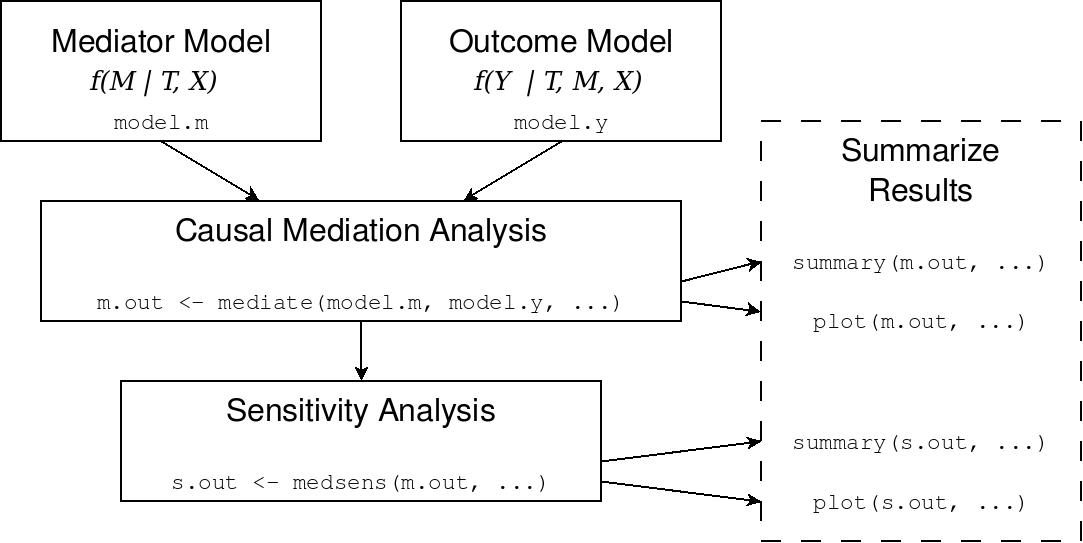
\includegraphics[scale=.35]{mediation-chart.jpg}
  \end{center}
  \caption{The Diagram Illustrating the Use of the Software
    \bmediation.  Users first fit the mediator and outcome models.
    Then, the function {\tt mediate} conducts causal mediation
    analysis while {\tt medsens} implements sensitivity analysis.  The
    functions {\tt summary} and {\tt plot} help users interpret the
    results of these analyses.} \label{fg:chart}
\end{figure}

Figure~\ref{fg:chart} graphically illustrates the three steps required
for a mediation analysis. The first step is to fit the mediator and
outcome models using, for example, regression models with the usual
\texttt{lm} or \texttt{glm} functions. In the second step, the
analysts takes the output objects from these models, which in
Figure~\ref{fg:chart} we call {\tt model.m} and {\tt model.y}, and use
them as inputs for the main function, {\tt mediate}. This function
then estimates the causal mediation effects, direct effects, and total
effect along with their uncertainty estimates. Finally, sensitivity
analysis can be conducted via the function {\tt medsens} which takes
the output of {\tt mediate} as an input.  For these outputs,
there are both {\tt summary} and {\tt plot} methods to
display numerical and graphical summaries of the analyses,
respectively.

\subsection{Estimation of the Causal Mediation Effects}

Estimation of the causal mediation effects is based on
Algorithms~1~and~2 of \citet{imai:keel:ting:10}. These are general
algorithms in that they can be applied to any parametric
(Algorithm~1~or~2) or semi/nonparametric models (Algorithm~2) for the
mediator and outcome variables.  Here, we briefly describe how these
algorithms have been implemented in \bmediation\ by taking advantage
of the object-oriented nature of \bR\ programming language.

\paragraph{Algorithm~1 for Parametric Models.}

We begin by explaining how to implement Algorithm~1 of
\citet{imai:keel:ting:10} for standard parametric models.  First,
analysts fit parametric models for the mediator and outcome
variables. That is, we model the observed mediator $M_i$ given the
treatment $T_i$ and pre-treatment covariates $X_i$.  Similarly, we
model the observed outcome $Y_i$ given the treatment, mediator, and
pre-treatment covariates.  For example, to implement the Baron-Kenny
procedure in \bmediation, linear models are fitted for both the
mediator and outcome models using the {\tt lm} command.

The model objects from these two parametric models form the inputs for
the {\tt mediate} function.  The user must also supply the names for
the mediator and outcome variables along with how many simulations
should be used for inference, and whether the mediator variable
interacts with the treatment variable in the outcome model.  Given
these model objects, the estimation proceeds by simulating the model
parameters based on their approximate asymptotic distribution (i.e.,
the multivariate normal distribution with the mean equal to the
parameter estimates and the variance equal to the asymptotic variance
estimate), and then computing causal mediation effects of interest for
each parameter draw (e.g., using
equations~\eqref{eq:acme}~and~\eqref{eq:direct} for average causal
mediation and (natural) direct effects, respectively).  This method of
inference can be viewed as an approximation to the Bayesian posterior
distribution due to the Bernstein-Von Mises Theorem
\citep{king:tomz:witt:00}.  The advantage of this procedure is that it
is relatively computationally efficient (when compared to
Algorithm~2).

We take advantage of the object-oriented nature of \bR\ programming
language at several steps in the function {\tt mediate}.  For
example, the functions like {\tt coef} and {\tt vcov} are useful
for extracting the point and uncertainty estimates from the model
objects to form the multivariate normal distribution from which the
parameter draws are sampled.  In addition, the computation of the
estimated causal mediation effects of interest requires the prediction
of the mediator values under different treatment regimes as well as
the prediction of the outcome values under different treatment and
mediator values.  This can be done by using {\tt model.frame} to set
the treatment and/or mediator values to specific levels while keeping
the values of the other variables unchanged.  We then use the {\tt
  model.matrix} and matrix multiplication with the distribution of
simulated parameters to compute the mediation and direct effects.  The
main advantage of this approach is that it is applicable to a wide
range of parametric models and allows us to avoid coding a completely
separate function for different models.

\paragraph{Algorithm~2 for Non/Semiparametric Inference.}

The disadvantage of Algorithm~1 is that it cannot be easily applied to
non/semiparametric models.  For such models, Algorithm~2, which is
based on nonparametric bootstrap, can be used although it is more
computationally intensive.  Algorithm~2 may also be used for the usual
parametric models which may be useful since mediation effects are
known to have skewed distributions
\citep[e.g.,][]{MacKinnon:2004,Preacher:Hayes:08}.  Specifically, in
Algorithm~2, we resample the observed data with replacement.  Then,
for each of bootstrapped samples, we fit both the outcome and mediator
models and compute the quantities of interest.  As before, the
computation requires the prediction of the mediator values under
different treatment regimes as well as the prediction of the outcome
values under different treatment and mediator values.  To take
advantage of the object-oriented nature of the \bR\ language,
Algorithm~2 relies on the \texttt{predict} function to compute these
predictions, while we again manipulate the treatment and mediator
status using the \texttt{model.frame} function. This process is
repeated a large number of times and returns a bootstrap distribution
of the mediation, direct, and total effects.  We use the percentiles
of the bootstrap distribution for confidence intervals. Thus,
Algorithm~2 allows analysts to estimate mediation effects with more
flexible model specifications or to estimate mediation effects for
quantiles of the distribution.

\subsection{Sensitivity Analysis}

Causal mediation analysis relies on the sequential ignorability
assumption that cannot be directly verified with the observed data.
The assumption implies that the treatment is ignorable given the
observed pre-treatment confounders and that the mediator is ignorable
given the observed treatment and the observed pre-treatment
covariates.  In order to probe the plausibility of such a key
identification assumption, analysts must perform a sensitivity
analysis \citep{rose:02c}.  Unfortunately, it is difficult to
construct a sensitivity analysis that is generally applicable to any
parametric or nonparametric model.  Thus,
\citet{imai:keel:yama:10,imai:keel:ting:10} develop sensitivity
analyses for commonly used parametric models, which we implement in
\bmediation.

\paragraph{The Baron-Kenny Procedure.}

\citet{imai:keel:yama:10} develop a sensitivity analysis for the
Baron-Kenny procedure and \citet{imai:keel:ting:10} generalize it to
the linear structural equation model (LSEM) with an interaction term.
This general model is given by,
\begin{eqnarray}
  M_i & = & \alpha_2 + \beta_2 T_i + \xi_2^\top X_i + \epsilon_{i2}, \label{eq:MgivenTX} \\
  Y_i & = & \alpha_3 + \beta_3 T_i + \gamma M_i + \kappa T_i M_i + \xi_3^\top X_i + \epsilon_{i3}, \label{eq:YgivenTMX}
\end{eqnarray}
where the sensitivity parameter is the correlation between
$\epsilon_{i2}$ and $\epsilon_{i3}$, which we denote by $\rho$.  Under
sequential ignorability, $\rho$ is equal to zero and thus the
magnitude of this correlation coefficient represents the departure
from the ignorability assumption (about the mediator).  Note that the
treatment is assumed to be ignorable as it would be the case in
randomized experiments where the treatment is randomized but the
mediator is not.  Theorem~2 of \citet{imai:keel:ting:10} shows how the
average causal mediation effects change as a function of $\rho$.

To obtain the confidence intervals for the sensitivity analysis, we
apply the following iterative algorithm to
equations~\eqref{eq:MgivenTX}~and~\eqref{eq:YgivenTMX} for a fixed
value of $\rho$.  At the $t$th iteration, given the current values of
the coefficients, i.e., $\theta^{(t)}=(\alpha_2^{(t)}, \beta_2^{(t)},
\xi_2^{(t)}, \alpha_3^{(t)},
\beta_3^{(t)},\xi_3^{(t)},\gamma^{(t)},\kappa^{(t)})$, and a given
error correlation $\rho$, we compute the variance-covariance matrix of
$(\epsilon_{i2},\epsilon_{i3})$, which is denoted by $\Sigma^{(t)}$.
The matrix is computed by setting
${\sigma_j^{(t)}}^2=\norm{\hat{\epsilon}_j^{(t)}}^2/(n-L_j)$ and
$\sigma_{23}^{(t)}=\rho \sigma_2^{(t)}\sigma_3^{(t)}$, where
$\hat\epsilon_j^{(t)}$ is the residual vector and $L_j$ is the number
of coefficients for the mediator model ($j=2$) and the outcome model
($j=3$) at the $t$th iteration.  We then update the parameters via
generalized least squares, i.e.,
\begin{eqnarray*}
  \theta^{(t+1)} & = & \{V^\top ({\Sigma^{(t)}}^{-1} \otimes I_n)V\}^{-1}
  V^\top ({\Sigma^{(t)}}^{-1} \otimes I_n)W
\end{eqnarray*}
where
$V  =  \l[\begin{array}{cccccccc} \mathbf{1} &  T & X & \mathbf{0} & \mathbf{0} & \mathbf{0} & \mathbf{0} & \mathbf{0} \\
  \mathbf{0} & \mathbf{0} & \mathbf{0} & \mathbf{1} & T & M & TM & X
\end{array} \r]$,
$W \ = \ \l[\begin{array}{c} M \\
  Y
\end{array} \r]$, $T=(T_1,\dots,T_n)^\top$, $M=(M_1,\dots,M_n)^\top$, and
$Y=(Y_1,\dots,Y_n)^\top$ are column vectors of length $n$, and $X = (X_1, \dots, X_n)^\top$ are the $(n \times K)$ matrix of observed pre-treatment covariates, and $\otimes$ represents the Kronecker product. We typically use
equation-by-equation least squares estimates as the starting values of $\theta$
and iterate these two steps until convergence.  This is essentially an
application of the iterative feasible generalized least square (FGLS) algorithm of the
seemingly unrelated regression \citep{zell:62}, and thus the asymptotic variance
of $\hat\theta$ is given by $\var(\hat\theta) = \{V^\top (\Sigma^{-1} \otimes
I_n) V\}^{-1}$. Then, for a given value of $\rho$, the asymptotic variance of the estimated average causal mediation effects
is found, for example, by the Delta method and the confidence intervals can be constructed.

\paragraph{The Binary Outcome Case.}

The sensitivity analysis for binary outcomes parallels the case when
both the mediator and outcome are continuous.  Here, we assume that
the model for the outcome is a probit regression. Using a probit
regression for the outcome allows us to assume the error terms are
jointly normal with a possibly non-zero correlation $\rho$.
\citet{imai:keel:ting:10} derive the average causal mediation effects
as a function of $\rho$ and a set of parameters that are identifiable
due to randomization of the treatment. This lets us use $\rho$ as a
sensitivity parameter in the same way as in the Baron-Kenny procedure.
For the calculation of confidence intervals, we rely on the
quasi-Bayesian approach of Algorithm~1 by approximating the posterior
distribution with the sampling distribution of the maximum likelihood
estimates.

% While it is possible to use a nonparametric bootstrap for the
% confidence intervals, it is much more computationally intensive.
% For a graphical summary of sensitivity analysis, we use a lowess
% smoother to smooth out sampling variability from the simulation when
% drawing the lines representing the point estimates and confidence
% intervals at a variety of $\rho$ values.

\paragraph{The Binary Mediator Case.}

Finally, a similar sensitivity analysis can also be conducted in a
situation where the mediator variable is dichotomous and the outcome
is continuous.  In this case, we assume that the mediator can be
modeled as a probit regression where the error term is independently
and identically distributed as standard normal distribution.  A linear
normal regression with error variance equal to $\sigma_3^2$ is used to
model the continuous outcome variable.  We further assume that the two
error terms jointly follow a bivariate normal distribution with mean
zero and covariance $\rho\sigma_3$.  Then, as in the other two cases,
we use the correlation between the two error terms $\rho$ as the
sensitivity parameter.  \citet{imai:keel:ting:10} show that under this
setup, the causal mediation effects can be expressed as a function of
the model parameters that can be consistently estimated given a fixed
value of $\rho$.  Uncertainty estimates are computed based on the
quasi-Bayesian approach, as in the binary outcome case.  The results
can be graphically summarized via the \texttt{plot} function in a
manner similar to the other two cases.

\paragraph{Alternative Interpretations Based on $R^2$}

The main advantage of using $\rho$ as a sensitivity parameter is its
simplicity.  However, applied researchers may find it difficult to
interpret the magnitude of this correlation coefficient.  To overcome
this limitation, \citet{imai:keel:yama:10} proposed alternative
interpretations of $\rho$ based on the coefficients of determination
or $R^2$ and \citet{imai:keel:ting:10} extended them to the binary
mediator and binary outcome cases.  In that formulation, it is assumed
that there exists a common unobserved pre-treament confounder in both
mediator and outcome models.  Applied researchers are then required to
specify whether the coefficients of this unobserved confounder in the
two models have the same sign or not; i.e.,
$\sgn(\lambda_2\lambda_3)=1$ or $-1$ where $\lambda_2$ and $\lambda_3$
are the coefficients in the mediator and outcome models, respectively.
Once this information is provided, the average causal mediation effect
can be expressed as the function of ``the proportions of original
variances explained by the unobserved confounder'' where the original
variances refer to the variances of the mediator and the outcome (or
the variance of latent variable in the case of binary dependent
variable).  This allows researchers to quantify how large the
unobserved confounder must be (relative to the observed pre-treatment
covariates in the model) in order for the original conclusions to be
reversed.

\paragraph{Sensitivity Analyses with Respect to the Average Direct Effects.}
In addition to the above procedures for the average causal mediation effects,
an analogous sensitivity analysis can also be conducted for the average direct
effects using the {\tt medsens} function.  This is possible because it can be
shown that the average direct effects are also expressed as a function of $\rho$
in any of the above three cases.  First, when both the mediator and outcome variables
are continuous and modelled using linear structural equations, the iterative FGLS algorithm
given above can be used to estimate the model coefficients and both the point and interval
estimates of the average direct effects can be obtained using the formulas given by
\citet[Section 4.1]{imai:keel:yama:10} and \citet[p.314 and Appendix A]{imai:keel:ting:10}.
Second, when the mediator is binary and modelled using the probit regression,
the average direct effect is given by $\bar\zeta(t) = \beta_3 + \kappa\E\{
\Phi(\alpha_2 + \beta_2 t + \xi_2^\top X_i)\}$ using the same notation as
\citet[footnote 12]{imai:keel:ting:10}, where all of the parameters, $(\alpha_2,
\beta_2, \xi_2, \beta_3, \kappa)$, are identified and consistently estimated
using the same procedure.  Finally, for the binary outcome case,
the average direct effect is identified given a value of $\rho$ and expressed
as $\bar\zeta(t) = \E\{\Phi(\alpha_1 + \beta_1 t + \xi_1^\top X_i +
\beta_3(1-t)/\sqrt{\gamma^2\sigma_2^2 + 2\gamma\rho\sigma_2 + 1})
- \Phi(\alpha_1 + \beta_1 t + \xi_1^\top X_i - \beta_3 t/\sqrt{\gamma^2\sigma_2^2 + 2\gamma\rho\sigma_2 + 1}) \}$, which can be estimated via the same procedure as
described in Appendix H of \citet{imai:keel:ting:10}.  The {\tt medsens} function
uses these procedures for sensitivity analyses for the average direct effects.

\subsection{Current Limitations}

\begin{table}[t]
 \spacingset{1}
  \begin{center}
\begin{tabular}{lcccccc}
\hline
                     &\multicolumn{6}{c}{\it Outcome Model Types} \\
\cline{2-7}
{\it Mediator Model Types} & Linear & GLM & Ordered & Censored & Quantile & Semiparametric \\
\hline
Linear ({\tt lm}) & \checkmark & \checkmark & \checkmark^\ast & \checkmark &
                                                  \checkmark & \checkmark^\ast  \\
GLM (probit etc. via {\tt glm})  & \checkmark & \checkmark & \checkmark^\ast & \checkmark &
                                                  \checkmark & \checkmark^\ast  \\
Ordered ({\tt polr}) & \checkmark & \checkmark & \checkmark^\ast & \checkmark &
                                                  \checkmark & \checkmark^\ast  \\
Censored (tobit via {\tt vglm}) & - & - & - & - & - & - \\
Quantile ({\tt rq}) & \checkmark^\ast & \checkmark^\ast & \checkmark^\ast & \checkmark^\ast &
                                                  \checkmark^\ast & \checkmark^\ast \\
Semiparametric ({\tt gam})   & \checkmark^\ast & \checkmark^\ast & \checkmark^\ast & \checkmark^\ast &
                                                  \checkmark^\ast & \checkmark^\ast \\
\hline
\end{tabular}
\caption{The Types of Models That Can be Handled by {\tt mediate} for the
  Estimation of Causal Mediation Effects. Asterisks ($^\ast$) indicate the model combinations
  that can only be estimated using the nonparametric bootstrap (i.e. with {\tt boot = TRUE}).} 
  \label{tab:MediateOptions}
  \end{center}
\end{table}

Our software, \bmediation, is quite flexible and can handle many of
the model types that researchers are likely to use in practice.
Table~\ref{tab:MediateOptions} categorizes the types of the mediator
and outcome models and lists whether \bmediation\ can produce the
point and uncertainty estimates of causal mediation effects. For
example, while \bmediation\ can estimate average causal mediation
effects for censored outcomes with the tobit model, it
has not yet been extended to cases involving censored mediators.
In each situation handled by \bmediation, it is possible to have an
interaction term between treatment status and the mediator variable,
in which case the estimated quantities of interest will be reported
separately for the treatment and control groups.

\begin{table}[t]
 \spacingset{1}
  \begin{center}
\begin{tabular}{lcc}
\hline
                     &\multicolumn{2}{c}{\it Outcome Model Types} \\
\cline{2-3}
{\it Mediator Model Types} & Linear & Binary Probit \\
\hline
Linear                     & \checkmark & \checkmark \\
Binary Probit              & \checkmark & - \\
\hline
\end{tabular}
\caption{The Types of Models That Can Be Handled by {\tt medsens} for
  Sensitivity Analysis. } \label{tab:SensitivityOptions}
  \end{center}
\end{table}

Our software provides a convenient way to probe the sensitivity of
results to potential violations of the ignorability assumption for
certain model types. The sensitivity analysis requires the specific
derivations for each combination of models, making it difficult to
develop a general sensitivity analysis method.  As summarized in
Table~\ref{tab:SensitivityOptions}, \bmediation\ can handle several
cases that are likely to be encountered by applied researchers in
practice. When the mediator is continuous, then sensitivity analysis
can be conducted with continuous and binary outcome variables.  In
addition, when the mediator is binary, sensitivity analysis is
available for continuous outcome variables.  For sensitivity analyses
that combine binary or continuous mediators and outcomes, analysts
must use a probit regression model with a linear regression model.
It should be noted that unlike the
estimation of causal mediation effects, sensitivity analysis with
treatment/mediator interactions can only be done for the continuous
outcome/continuous mediator and continuous outcome/binary mediator cases.
In the future, we hope to expand the range of models that
are available for sensitivity analysis.

\section{Examples}

Next, we provide several examples to illustrate the use of
\bmediation\ for the estimation of causal mediation effects and
sensitivity analysis.  The data used is available as part of the
package so that readers can replicate the results reported below.  We
demonstrate the variety of models that can be used for the outcome and
mediating variables.

Before presenting our examples, we load the \bmediation\ library and
the example data set included with the library.
\begin{verbatim}
R> library("mediation")
mediation: R Package for Causal Mediation Analysis
Version: 2.0
R> data("jobs")
\end{verbatim}
This dataset is from the Job Search Intervention Study (JOBS II)
\citep{Vinokur:1997}. In the JOBS II field experiment, 1,801
unemployed workers received a pre-screening questionnaire and were
then randomly assigned to treatment and control groups. Those in the
treatment group participated in job-skills workshops.  Those in the
control condition received a booklet describing job-search tips. In
follow-up interviews, two key outcome variables were measured; a
continuous measure of depressive symptoms based on the Hopkins Symptom
Checklist (\texttt{depress2}), and a binary variable representing
whether the respondent had become employed (\texttt{work1}). In the
JOBS II data, a continuous measure of job-search self-efficacy
represents a key mediating variable (\texttt{job\_seek}). In addition
to the outcome and mediators, the JOBS II data also include the
following list of baseline covariates that were measured prior to the
administration of the treatment: pre-treatment level of depression
(\texttt{depress1}), education (\texttt{educ}), income, race
(\texttt{nonwhite}), marital status (\texttt{marital}), age, sex,
previous occupation (\texttt{occp}), and the level of economic
hardship (\texttt{econ\_hard}).

\subsection{Estimation of Causal Mediation Effects}

\paragraph{The Baron-Kenny Procedure.}
We start with an example when both the mediator and the outcome are
continuous.  In this instance, the results from either algorithm will
return point estimates essentially identical to the usual Baron and
Kenny procedure though the quasi-Bayesian or nonparametric bootstrap
approximation is used.  Using the JOBS II data, we first estimate two
linear regressions for both the mediator and the outcome using the {\tt
lm} function.
\begin{verbatim}
R> model.m <- lm(job_seek ~ treat + depress1 + econ_hard + sex + age
                  + occp + marital + nonwhite + educ + income, data = jobs)
R> model.y <- lm(depress2 ~ treat + job_seek + depress1 + econ_hard + sex + age
                  + occp + marital + nonwhite + educ + income, data = jobs)
\end{verbatim}
These two model objects, {\tt model.m} and {\tt model.y}, become the
arguments for the \texttt{mediate} function.  When different data frames
are used for these two models, the {\tt mediate} function internally refits
them using a merged dataset if the {\tt dropobs} argument is set to
{\tt TRUE}; otherwise an error message is returned.

In the first call to \texttt{mediate} below, we specify \texttt{boot
  = TRUE} to call the nonparametric bootstrap with 1000 resamples
({\tt sims = 1000}). When this option is set to {\tt FALSE} in the second
call, inference proceeds via the quasi-Bayesian Monte Carlo
approximation using Algorithm~1 rather than Algorithm~2.  In this case,
heteroskedasticity-robust standard errors can be used for the calculation of
confidence intervals for some types of models by setting the {\tt robustSE}
argument to {\tt TRUE}.  Finally, we must also
specify the variable names for the treatment indicator and the
mediator variable using {\tt treat} and {\tt mediator}, respectively.
\begin{verbatim}
R> out.1 <- mediate(model.m, model.y, sims = 1000, boot = TRUE, treat = "treat",
                    mediator = "job_seek")
R> out.2 <- mediate(model.m, model.y, sims = 1000, treat = "treat",
                    mediator = "job_seek")
\end{verbatim}
The objects from a call to \texttt{mediate}, i.e., {\tt out.1} and
{\tt out.2} above, are lists of class {\tt "mediate"} which contain several different
quantities from the analysis.  For example, \texttt{out.1\$d0} returns
the point estimate for the average causal mediation effect based on
Algorithm~1.  The help file contains a full list of values that are
contained in \texttt{mediate} objects.

The \texttt{summary}
function prints out the results of the analysis in tabular form:
\begin{verbatim}
R> summary(out.2)

 Causal Mediation Analysis

Quasi-Bayesian Confidence Intervals

Mediation Effect:  -0.01385 95 % CI  -0.033175  0.002333
Direct Effect:  -0.03879 95 % CI  -0.11989  0.04682
Total Effect:  -0.05264 95 % CI  -0.13324  0.03459
Proportion of Total Effect via Mediation:  0.2146 95 % CI  -1.387  1.906

Sample Size Used: 899
\end{verbatim}
The output from the {\tt summary} function displays the estimates
for the average causal mediation effect, direct effect, total effect,
and proportion of total effect mediated. The first column displays the
quantity of interest, the second column displays the point estimate,
and the other columns present the confidence intervals at the level
specified by the {\tt conf.level} argument which defaults to {\tt 0.95}.
The number of observations used for the estimation is then displayed at
the bottom.  In this case, we
find that job search self-efficacy mediated the effect of the
treatment on depression in the negative direction. This effect,
however, was small with a point estimate of $-.014$ and the $95\%$
confidence interval $(-.033,-.002)$ barely covers $0$.

These results can be graphically presented by using the {\tt plot} function:
\begin{verbatim}
R> plot(out.2)
\end{verbatim}
The output is shown in Figure~\ref{fig:plot.mediate}. The standard arguments
for {\tt plot}, such as titles ({\tt main}, {\tt xlab}, etc.) and line widths 
({\tt lwd}), can be used and behave as expected.

\begin{figure}[t]
\spacingset{1}
\vspace{-.5in}
\begin{center}
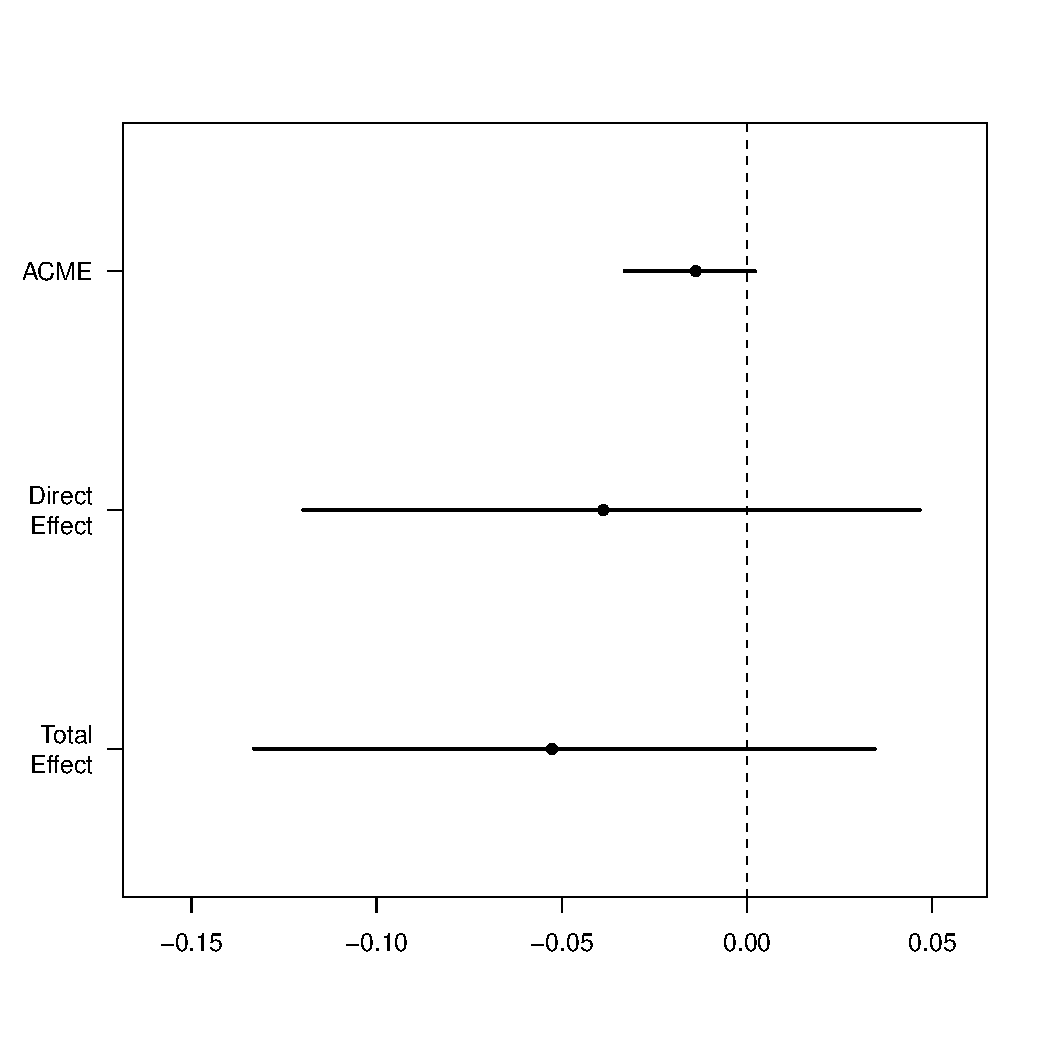
\includegraphics[scale=.8]{plot-mediate.pdf}
\end{center}
\vspace{-.5in}
\caption{Graphical Summary of Causal Mediation Analysis.
  \label{fig:plot.mediate}}
\end{figure}

\paragraph{The Baron-Kenny Procedure with the Interaction Term.}
Analysts can also allow the causal mediation effect to vary with
treatment status.  Here, the model for the outcome must be altered by
including an interaction term between the treatment indicator,
\texttt{treat}, and the mediator variable, \texttt{job\_seek}:
\begin{verbatim}
R> model.y <- lm(depress2 ~ treat + job_seek + treat:job_seek + depress1 + econ_hard
               + sex + age + occp + marital + nonwhite + educ + income, data = jobs)
R> out.3 <- mediate(model.m, model.y, sims = 1000, boot = TRUE,
                    treat = "treat", mediator = "job_seek")
R> summary(out.3)

 Causal Mediation Analysis

Quasi-Bayesian Confidence Intervals

Mediation Effect_0:  -0.01829 95 % CI  -0.046754  0.005477
Mediation Effect_1:  -0.01164 95 % CI  -0.027492  0.003419
Direct Effect_0:  -0.03577 95 % CI  -0.1170  0.0420
Direct Effect_1:  -0.02912 95 % CI  -0.10900  0.05012
Total Effect:  -0.04741 95 % CI  -0.13040  0.03249
Proportion of Total Effect via Mediation_0:  0.2821 95 % CI  -2.254  3.517
Proportion of Total Effect via Mediation_1:  0.1801 95 % CI  -1.535  2.253

Mediation Effect (Average):  -0.01496 95 % CI  -0.034988  0.004684
Direct Effect (Average):  -0.03245 95 % CI  -0.11272  0.04712
Proportion of Total Effect via Mediation (Average):  0.2321 95 % CI  -1.889  2.860

Sample Size Used: 899
\end{verbatim}
Again using the \texttt{summary} function provides a table of the
results. Now estimates for the mediation effects, direct effects and
proportion of totel effect mediated correspond
to the levels of the treatment and are printed as such in the tabular
summary.  In this case, the mediation effect under the treatment
condition, listed as \texttt{Mediation Effect\_1} is estimated to be
$-.012$ while the mediation effect under the control condition,
\texttt{Mediation Effect\_0}, is $-.018$.  The bottom of the table shows
the overall summary of these quantities averaged over the two treatment levels,
as well as the number of data points.

When using the {\tt plot} function on a {\tt mediate} object with interactions,
one can select which treatment condition to plot the estimated effects for by
specifying the {\tt treatment} argument.  The default is to plot both estimates,
which is equivalent to setting {\tt treatment} to {\tt "both"}:
\begin{verbatim}
R> plot(out.3, treatment = "both")
\end{verbatim}
The resulting plot is in Figure~\ref{fig:plot.mediate.int}.

\begin{figure}[t]
\spacingset{1}
\vspace{-.5in}
\begin{center}
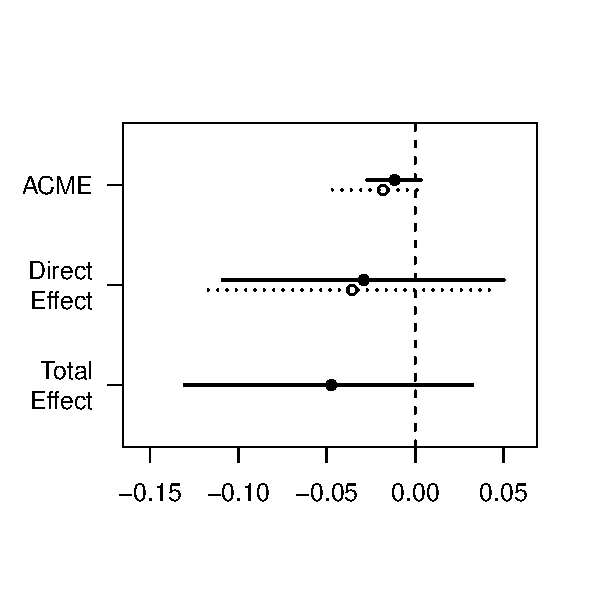
\includegraphics[scale=.8]{plot-mediate-int.pdf}
\end{center}
\vspace{-.5in}
\caption{Causal Mediation Analysis with Interaction
between Treatment and Mediator.
  \label{fig:plot.mediate.int}}
\end{figure}


\paragraph{Use of Non/Semi-parametric Regression.}

The flexibility of \bmediation\ becomes readily apparent when we move
beyond standard linear regression models.  For example, we might
suspect that the mediator has a nonlinear effect on the outcome.
Generalized Additive Models (GAMs) allow analysts to use splines for
flexible nonlinear fits.  This presents no difficulties for the
\texttt{mediate} function.  We model the mediator as before, but we
alter the outcome model using the \texttt{gam} function from the
\texttt{mgcv} library.
\begin{verbatim}
R> model.m <- lm(job_seek ~ treat + depress1 + econ_hard + sex + age + occp + marital
                 + nonwhite + educ + income, data = jobs)
R> model.y <- gam(depress2 ~ treat + s(job_seek, bs = "cr")  + depress1 + econ_hard
                 + sex + age + occp + marital + nonwhite + educ + income, data = jobs)
\end{verbatim}
In this case we fit a Generalized Additive Model for the outcome
variable, but allow the effect of the \texttt{job\_seek} variable to
be non-linear and determined by the data. This is done by using the
\texttt{s} notation which allows the fit between the mediator and
the outcome to be modeled with a spline.  Using the spline for the fit
allows the estimate for the mediator on the outcome to be a series of
piecewise polynomial regression fits. This semiparametric regression
model is a more general version of nonparametric regression models
such as lowess. The model above allows the estimate to vary across the
range of the predictor variable. Here, we specify the model with a
cubic basis function (\texttt{bs = "cr"}) for the smoothing spline and
leave the smoothing selection to be done at the program defaults which
is generalized cross-validation.  Fully understanding how to fit such
models is beyond the scope here.  Interested readers should consult
\cite{Wood:2006} for full technical details and \cite{Keele:2008}
provides coverage of these models from a social science perspective.

The call to \texttt{mediate} with a \texttt{gam} fit remains
unchanged except that when the outcome model is a semiparametric
regression only the nonparametric bootstrap is valid for calculating
uncertainty estimates, i.e., {\tt boot = TRUE}.
\begin{verbatim}
R> out.4 <- mediate(model.m, model.y, sims = 1000, boot = TRUE, treat = "treat",
                    mediator = "job_seek")
\end{verbatim}

The model for the mediator can be modeled with the \texttt{gam}
function as well.  The \texttt{gam} function also allows analysts to
include interactions; thus analysts can still allow the mediation
effects to vary with treatment status.  This simply requires altering
the model specification by using the \texttt{by} option in the
\texttt{gam} function and using two separate indicator variables for
treatment status.  To fit this model we need one variable that
indicates whether the observation was in the treatment group and a
second variable that indicates whether the observation was in the
control group.  To allow the mediation effect to vary with treatment
status, the call to \texttt{gam} takes the following form:
\begin{verbatim}
R> model.y <- gam(depress2 ~ treat + s(job_seek, by = treat) + s(job_seek, by = control)
         + depress1 + econ_hard + sex + age + occp + marital + nonwhite + educ + income,
         data = jobs)
\end{verbatim}
In this case, we must also alter the options in the \texttt{mediate}
function by providing the variable
name for the control group indicator using the \texttt{control} option.
\begin{verbatim}
R> out.5 <- mediate(model.m, model.y, sims = 1000, boot = TRUE,
                    treat = "treat", mediator = "job_seek", control = "control")
R> summary(out.5)

 Causal Mediation Analysis 

Confidence Intervals Based on Nonparametric Bootstrap

Mediation Effect_0:  -0.02285 95 % CI  -0.052889  0.003819 
Mediation Effect_1:  -0.01710 95 % CI  -0.039015  0.002544 
Direct Effect_0:  -0.01093 95 % CI  -0.09689  0.07581 
Direct Effect_1:  -0.005191 95 % CI  -0.08789  0.07816 
Total Effect:  -0.02804 95 % CI  -0.11704  0.06002 
Proportion of Total Effect via Mediation_0:  0.3817 95 % CI  -4.315  6.295 
Proportion of Total Effect via Mediation_1:  0.2742 95 % CI  -3.915  4.472 

Mediation Effect (Average):  -0.01998 95 % CI  -0.045832  0.003162 
Direct Effect (Average):  -0.008063 95 % CI  -0.09149  0.07672 
Proportion of Total Effect via Mediation (Average):  0.3237 95 % CI  -4.053  5.166 

Sample Size Used: 899 
\end{verbatim}

\paragraph{Quantile Causal Mediation Effects.}

Researchers might also be interested in modeling mediation effects for
quantiles of the outcome.  Quantile regression allows for a convenient
way to model the quantiles of the outcome distribution while adjusting
for a variety of covariates \citep{Koenker:2005}.  For example, a
researcher might be interested in the 0.5 quantile (i.e., median)
of the distribution. This also presents no difficulties for the
\texttt{mediate} function.  Again for these models, uncertainty
estimates are calculated using the nonparametric bootstrap.  To use
quantile regression, we use the {\tt rq} function in package 
\texttt{quantreg} and model
the median of the outcome, though other quantiles are also
permissible.  Analysts can also relax the no-interaction assumption
for the quantile regression models as well.  Below we estimate the
mediator with a standard linear regression, while for the outcome we
use \texttt{rq} to model the median.
\begin{verbatim}
R> model.m <- lm(job_seek ~ treat + depress1 + econ_hard + sex + age + occp + marital
                 + nonwhite + educ + income, data = jobs)
R> model.y <- rq(depress2 ~ treat + job_seek + depress1 + econ_hard + sex
                 + age + occp + marital + nonwhite + educ + income, 
                 tau = 0.5, data = jobs)
R> out.6 <- mediate(model.m, model.y, sims = 1000, boot = TRUE, treat = "treat",
                    mediator = "job_seek")
R> summary(out.6)

 Causal Mediation Analysis 

Confidence Intervals Based on Nonparametric Bootstrap

Mediation Effect:  -0.01426 95 % CI  -0.031162  0.002092 
Direct Effect:  -0.04152 95 % CI  -0.12300  0.03562 
Total Effect:  -0.05577 95 % CI  -0.14335  0.02364 
Proportion of Total Effect via Mediation:  0.2000 95 % CI  -2.866  2.300 

Sample Size Used: 899 
\end{verbatim}
where the {\tt summary} command gives the estimated median causal
mediation effect along with the estimates for the other quantities of
interest.

It is also possible to estimate mediation effects for quantiles of the
outcome other than the median. This is done simply by specifying a
different outcome quantile in the quantile regression model. For
example, if the $10th$ percentile of the outcome were of interest,
then the user can change {\tt tau} option,
\begin{verbatim}
R> model.y <- rq(depress2 ~ treat + job_seek + depress1 + econ_hard + sex
                 + age + occp + marital + nonwhite + educ + income, 
                 tau = 0.1, data = jobs)
\end{verbatim}
Furthermore, it is straightforward to loop over a set of quantiles and
graph the mediation effects for a range of quantiles, as done in
\citet{imai:keel:ting:10}.

\paragraph{Discrete Mediator and Outcome Data.}

Often analysts use measures for the mediator and outcome that are
discrete.  For standard methods, this has presented a number of
complications requiring individually tailored techniques.  The
\bmediation\ software, however, can handle a number of different
discrete data types using the general algorithms developed in
\citet{imai:keel:ting:10}.  For example, one outcome of interest in
the JOBS II study is a binary indicator (\texttt{work1}) for whether
the subject became employed after the training sessions. To estimate
the mediation effect, we simply use a probit regression instead of a
linear regression for the outcome and then call \texttt{mediate} as
before,
\begin{verbatim}
R> model.m <- lm(job_seek ~ treat + depress1 + econ_hard + sex + age 
                + occp + marital + nonwhite + educ + income, data = jobs)
R> model.y <- glm(work1 ~ treat + job_seek + depress1 + econ_hard + sex + age 
                + occp + marital + nonwhite + educ + income, 
                family = binomial(link = "probit"), data = jobs)
R> out.7 <- mediate(model.m, model.y, sims = 1000, treat = "treat",
                    mediator = "job_seek")
R> summary(out.7)

 Causal Mediation Analysis 

Quasi-Bayesian Confidence Intervals

Mediation Effect_0:  0.003340 95 % CI  -0.0009266  0.0101511 
Mediation Effect_1:  0.003588 95 % CI  -0.001001  0.010833 
Direct Effect_0:  0.05592 95 % CI  -0.004395  0.116298 
Direct Effect_1:  0.05617 95 % CI  -0.004405  0.116453 
Total Effect:  0.05951 95 % CI  -0.0006978  0.1196860 
Proportion of Total Effect via Mediation_0:  0.04671 95 % CI  -0.06537  0.40433 
Proportion of Total Effect via Mediation_1:  0.05055 95 % CI  -0.06854  0.40859 

Mediation Effect (Average):  0.003464 95 % CI  -0.0009614  0.0105733 
Direct Effect (Average):  0.05604 95 % CI  -0.0044  0.1164 
Proportion of Total Effect via Mediation (Average):  0.0484 95 % CI  -0.06695  0.40646 

Sample Size Used: 899 
\end{verbatim}

In the table printed by the \texttt{summary} function, the estimated
average causal mediation effect along with the quasi-Bayesian
confidence interval are printed on the first line followed by the
direct and total effects, and the proportion of the total effect due
to mediation.  Even though the outcome model does not include an interaction
term between the treatment and mediator, the estimated effects slightly differ
between the treatment and control conditions.  This difference, however, 
is solely due to the nonlinearity in the outcome model and should be
extremely small.  It is also possible to use a logit model for the
outcome instead of a probit model.  However, we recommend the use of a
probit model because our implementation of the sensitivity analysis
below requires a probit model for analytical tractability.

The mediator can also be binary or ordered measures as well.  This
simply requires modeling the mediator with either a probit or ordered
probit model.  For demonstration purposes, the \texttt{jobs} data
contains two variables, \texttt{job\_dich} and \texttt{job\_disc},
which are recoded versions of \texttt{job\_seek}.  The first measure
is simply the continuous scale divided at the median into a binary
variable.  The second measure, \texttt{job\_disc}, recodes the
continuous scale into a discrete four point scale.  We emphasize that
this is for demonstration purposes only, and analysts in general
should not recode continuous measures into discrete measures.
Estimating mediation effects with a binary mediator is quite similar
to the case above with a binary outcome.  We simply now use a probit
model for the mediator and a linear regression for the outcome,
\begin{verbatim}
R> model.m <- glm(job_dich ~ treat + depress1 + econ_hard + sex + age
                + occp + marital + nonwhite + educ + income, data = job, 
                family = binomial(link = "probit"))
R> model.y <- lm(depress2 ~ treat + job_dich + treat:job_dich + depress1
                + econ_hard + sex + age + occp + marital + nonwhite 
                + educ + income, data = jobs)
\end{verbatim}

In this example we include the interaction term between the treatment and
mediator to allow the effect of the mediator to vary with
treatment status.  The user now calls \texttt{mediate} and can use
either the quasi-Bayesian approximation or nonparametric bootstrap.
\begin{verbatim}
R> out.8 <- mediate(model.m, model.y, sims = 1000, treat = "treat",
                    mediator = "job_dich")
R> summary(out.8)
 Causal Mediation Analysis 

Quasi-Bayesian Confidence Intervals

Mediation Effect_0:  -0.01815 95 % CI  -0.037383 -0.003393 
Mediation Effect_1:  -0.02035 95 % CI  -0.039359 -0.003966 
Direct Effect_0:  -0.03076 95 % CI  -0.11109  0.04833 
Direct Effect_1:  -0.03296 95 % CI  -0.11524  0.04722 
Total Effect:  -0.05111 95 % CI  -0.12946  0.03085 
Proportion of Total Effect via Mediation_0:  0.2695 95 % CI  -2.430  3.154 
Proportion of Total Effect via Mediation_1:  0.3135 95 % CI  -2.906  3.379 

Mediation Effect (Average):  -0.01925 95 % CI  -0.035705 -0.004607 
Direct Effect (Average):  -0.03186 95 % CI  -0.11337  0.04748 
Proportion of Total Effect via Mediation (Average):  0.301 95 % CI  -2.496  2.757 

Sample Size Used: 899 
\end{verbatim}

\noindent In the table, we see that \texttt{Mediation Effect\_0} is
the mediation effect under the control condition, while
\texttt{Mediation Effect\_1} is the mediation effect under the
treatment condition.  The same notation applies to the direct effects.
As the reader can see, the output also indicates which algorithm is
used for the 95\% confidence intervals.

When the mediator is an ordered variable, we switch to an ordered
probit model for the mediator.  In \bR, the \texttt{polr} function
in the \texttt{MASS} library provides this functionality.  Thus, we
fit the outcome and mediator models below,
\begin{verbatim}
R> model.m <- polr(job_disc ~ treat + depress1 + econ_hard + sex + age 
                + occp + marital + nonwhite + educ + income, 
                data = jobs, method = "probit", Hess = TRUE)
R> model.y <- lm(depress2 ~ treat + job_disc + depress1 + econ_hard + sex + age 
                + occp + marital + nonwhite + educ + income, data = jobs)
\end{verbatim}
The reader should note that in the call to \texttt{polr} the
\texttt{Hess = TRUE} should be specified to compute the asymptotic variance
covariance matrix for the estimated model coefficients in the quasi-Bayesian
approximation.  Otherwise, the Hessian of the log-likelihood will be recalculated
within the {\tt mediate} call.  

Once we have estimated these two models, analysis proceeds as before,
\begin{verbatim}
R> out.9 <- mediate(model.m, model.y, sims = 1000, treat = "treat",
                     mediator = "job_disc")
R> summary(out.9)
\end{verbatim}
Again, for any of these data types, analysts can relax the
no-interaction assumption as before by including the interaction
between treatment and the mediator variable in the outcome model.

\subsection{Sensitivity Analysis}

Once analysts have estimated mediation effects, they should explore how 
robust their finding is to the ignorability assumption, whenever possible.
The \texttt{medsens} function allows analysts to conduct sensitivity
analyses for mediation effects as well as direct effects.  
In this section we provide a demonstration of these functionalities.
Currently, \bmediation\ can conduct sensitivity analyses when both mediator
and outcome are continuous and modelled with the {\tt lm} function, as well
as when either mediator or outcome (but not both) is binary and modelled using
a binary probit regression via {\tt glm}.

\paragraph{The Baron-Kenny Procedure.}
As before, one must first fit models for the mediator and outcome and then pass these model objects through the mediate function:
\begin{verbatim}
R> model.m <- lm(job_seek ~ treat + depress1 + econ_hard + sex + age + occp 
                + marital + nonwhite + educ + income, data = jobs)
R> model.y <- lm(depress2 ~ treat + job_seek + depress1 + econ_hard + sex + age + occp
                + marital + nonwhite + educ + income, data = jobs)
R> med.cont <- mediate(model.m, model.y, sims=1000,  treat = "treat",
                       mediator = "job_seek")
\end{verbatim}

Once the analyst estimates the mediation effects, the output from the
{\tt mediate} function becomes the argument for \texttt{medsens},
which is the workhorse function. The {\tt medsens} function
recognizes main arguments specified in the {\tt mediate} function and
thus there is no need to specify options such as \texttt{treat} or 
\texttt{mediator}.
\begin{verbatim}
R> sens.cont <- medsens(med.cont, rho.by = 0.05)
\end{verbatim}
The \texttt{rho.by} option specifies how finely incremented the parameter $\rho$
is for the sensitivity analysis. When $\rho$ is on a coarser grid, this speeds
up estimation considerably but comes at the cost of estimating the
robustness of the original conclusion only imprecisely.

After running the sensitivity analysis via \texttt{medsens}, the
\texttt{summary} function can be used to produce a table with the
values of $\rho$ for which the confidence interval contains zero.
This allows the analyst to immediately see the approximate range of
$\rho$ where the sign of the causal mediation effect is indeterminate.
The second section of the table contains the value of $\rho$ for which
the mediation effect is exactly zero, which in this application is
$-0.19$. The table also presents coefficients of determination that
correspond to the critical value of $\rho$ where the mediation effect
is zero. First, ${R^\ast}^2_M{R^\ast}^2_Y$ is the product of
coefficients of determination which represents the proportion of the
\emph{previously unexplained} variance in the mediator and outcome
variables that is explained by an unobservable pretreatment
unconfounder.  An alternative formulation is in terms of the
proportion of the \emph{original} variance explained by an unobserved
confounder, which we denote as $\widetilde{R}^2_M\widetilde{R}^2_Y$ .
\begin{verbatim}
R> summary(sens.cont)

Mediation Sensitivity Analysis

Sensitivity Region

       Rho Med. Eff. 95% CI Lower 95% CI Upper R^2_M*R^2_Y* R^2_M~R^2_Y~
[1,] -0.25    0.0056      -0.0008       0.0120       0.0625       0.0403
[2,] -0.20    0.0012      -0.0035       0.0058       0.0400       0.0258
[3,] -0.15   -0.0032      -0.0084       0.0020       0.0225       0.0145
[4,] -0.10   -0.0074      -0.0150       0.0001       0.0100       0.0064

Rho at which ACME = 0: -0.1867

R^2_M*R^2_Y* at which ACME = 0: 0.0349

R^2_M~R^2_Y~ at which ACME = 0: 0.0225

\end{verbatim}
The table above presents the estimated mediation effect along with its
confidence interval for each value of $\rho$.  The reader can verify
that when $\rho$ is equal to zero, the reported mediation effect
matches the estimate produced by the \texttt{mediate} function.  For
other values of $\rho$, the mediation effect is calculated under
different levels of unobserved confounding.

The information from the sensitivity analysis can also be summarized
graphically using the \texttt{plot} function.  First, passing the
\texttt{medsens} object to \texttt{plot} and specifying the
\texttt{sens.par} option to \texttt{"rho"}, i.e.,
\begin{verbatim}
R> plot(sens.cont, sens.par = "rho")
\end{verbatim}
produces the left hand side of Figure~\ref{jobplot1}.  In the plot, the dashed
horizontal line represents the estimated mediation effect under the sequential
ignorability assumption, and the solid line represents the mediation
effect under various values of $\rho$.  The grey region represents the
95\% confidence bands.

Similarly, we can also plot the sensitivity analysis in terms of the
coefficients of determination as discussed above. Here we specify \texttt{sens.par}
option to \texttt{"R2"}.  We also need to specify two additional pieces of information.
First, \texttt{r.type} option tells the plot function whether to plot
${R^\ast}^2_M{R^\ast}^2_Y$ or $\widetilde{R}^2_M\widetilde{R}^2_Y$. To plot the
former \texttt{r.type} is set to \texttt{"residual"} and to plot the latter 
\texttt{r.type} is set
to \texttt{"total"}.  Finally, the \texttt{sign.prod} option specifies the sign of the
product of the coefficients of the unobserved confounder in the mediator and outcome models.
This product indicates whether the unobserved confounder affects both mediator and outcome
variables in the same direction (\texttt{"positive"}) or different directions 
(\texttt{"negative"}), thereby
reflecting the analyst's expectation about the nature of confounding.

For example, the following command produces the plot representing the sensitivity
of estimates with respect to the proportion of the original variances explained by
the unobserved confounder when the confounder is hypothesized to affect the mediator
and outcome variables in opposite directions.
\begin{verbatim}
R> plot(sens.cont, sens.par = "R2", r.type = "total", sign.prod = "negative")
\end{verbatim}
The resulting plot is shown on the right hand side of Figure~\ref{jobplot1}. Each contour
line represents the mediation effect for the corresponding values of
$\widetilde{R}^2_M$ and $\widetilde{R}^2_Y$. For example, the 0 contour line
corresponds to values of the product $\widetilde{R}^2_M\widetilde{R}^2_Y$ such
that the ACME is 0. As reported in the table, even a small proportion of
original variance unexplained by the confounder, $.02\%$, produces mediation
effects of 0.  Accordingly, the right hand side of Figure~\ref{jobplot1} shows
how increases in $\widetilde{R}^2_M\widetilde{R}^2_Y$ (moving from the lower
left to upper right) produce \emph{positive} mediation effects.

For both types of sensitivity plots, the user can specify additional options
available in the plot function such as alternative
title (\texttt{main}) and axis labels (\texttt{xlab}, \texttt{ylab}) or
manipulate common graphical options (e.g., \texttt{xlim}).


\begin{figure}[t]
\spacingset{1}
\vspace{-.5in}
\begin{center}
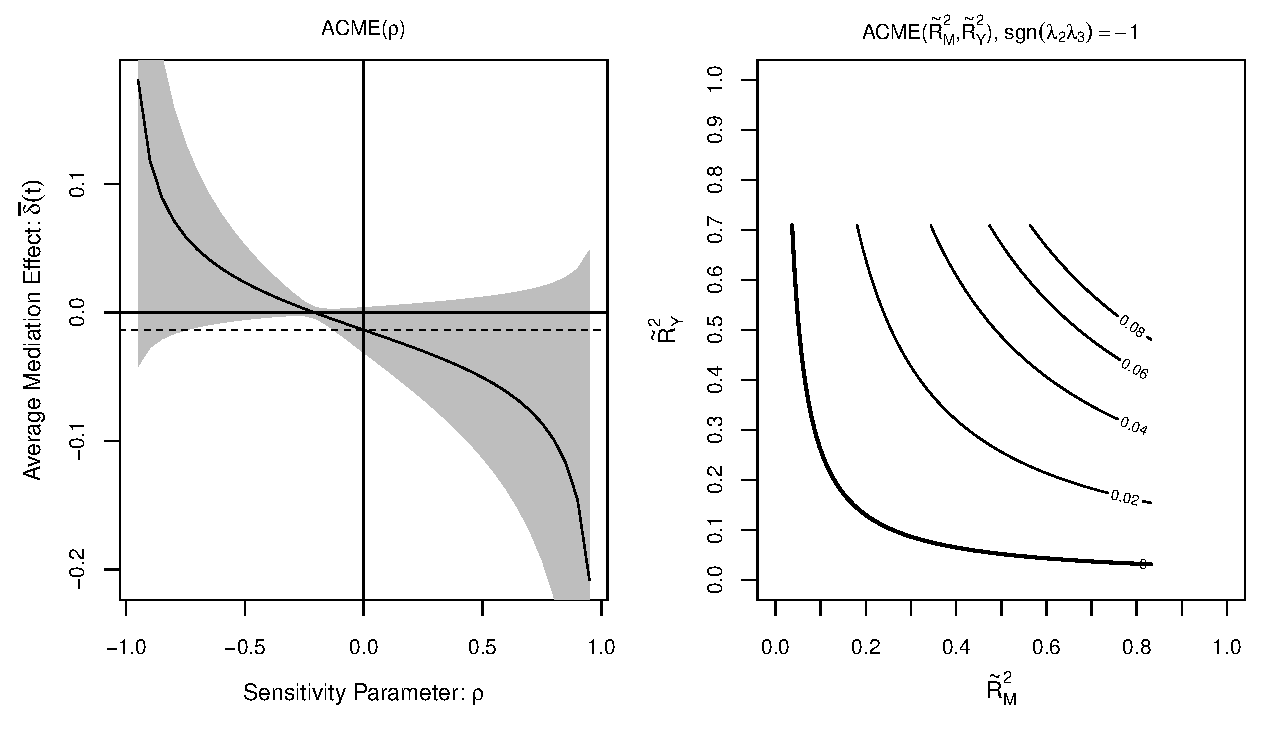
\includegraphics[scale=.8]{Rho-R2-ContCont-JOBS.pdf}
\end{center}
\vspace{-.5in}
\caption{Sensitivity Analysis with Continuous Outcome and Mediator.
  \label{jobplot1}}
\end{figure}


\paragraph{Binary Outcome.}

The \texttt{medsens} function also extends to analyses where the
mediator is binary and the outcome is continuous, as well as when the
mediator is continuous and the outcome is binary.  If either variable
is binary, \texttt{medsens} takes an additional argument.  For
example, recall the binary outcome model estimated earlier:
\begin{verbatim}
R> model.y <- glm(work1 ~ treat + job_seek + depress1 + econ_hard + sex + age 
                + occp + marital + nonwhite + educ + income, 
                family = binomial(link = "probit"), data = jobs)
R> med.bout <- mediate(model.m, model.y, sims = 1000, treat = "treat",
                       mediator = "job_seek")
\end{verbatim}

The call to \texttt{medsens} works as before, with the output from the \texttt{mediate}
function passed through \texttt{medsens}.
\begin{verbatim}
R> sens.bout <- medsens(med.bout, rho.by = 0.05, sims = 1000)
\end{verbatim}
The \texttt{sims} option provides control over the number of Monte Carlo draws 
used to compute confidence bands.
When either the mediator or outcome is binary, the exact values of
sensitivity parameters where the mediation effects are zero cannot be analytically
obtained as in the fully continuous case \citep[see][Section 4]{imai:keel:yama:10}.
Thus, this information is reported based on the signs of the estimated mediation
effects under various values of $\rho$ and corresponding coefficients of determination.
The usage of the \texttt{summary} function, however, remains
identical to the fully continuous case
in that the output table contains the estimated mediation
effects and the corresponding values of $\rho$ for which the
confidence region contains zero.

As in the case with continuous mediator and outcome variables, we can plot the
results of the sensitivity analysis.  The following code produces Figure~\ref{SensBinOut}.
\begin{verbatim}
R> plot(sens.bout, sens.par = "rho")
R> plot(sens.bout, sens.par = "R2", r.type = "total", sign.prod = "positive")
\end{verbatim}
On the left hand side we plot the ACME in terms of $\rho$, while we plot the ACME
in terms of $\widetilde{R}^2_M$ and $\widetilde{R}^2_Y$ on the right hand side.
In the $\rho$ plot, the dashed line represents the estimated mediation effect
under sequential
ignorability, and the solid line represents the mediation effect under
various values of $\rho$.  The grey region represents the 95\%
confidence bands. In the $\widetilde{R}^2$ plot the ACME is plotted against various values of $\widetilde{R}^2_M$ and $\widetilde{R}^2_Y$ and is interpreted in the same way as above.

\begin{figure}[t]
\spacingset{1}
\vspace{-.5in}
\begin{center}
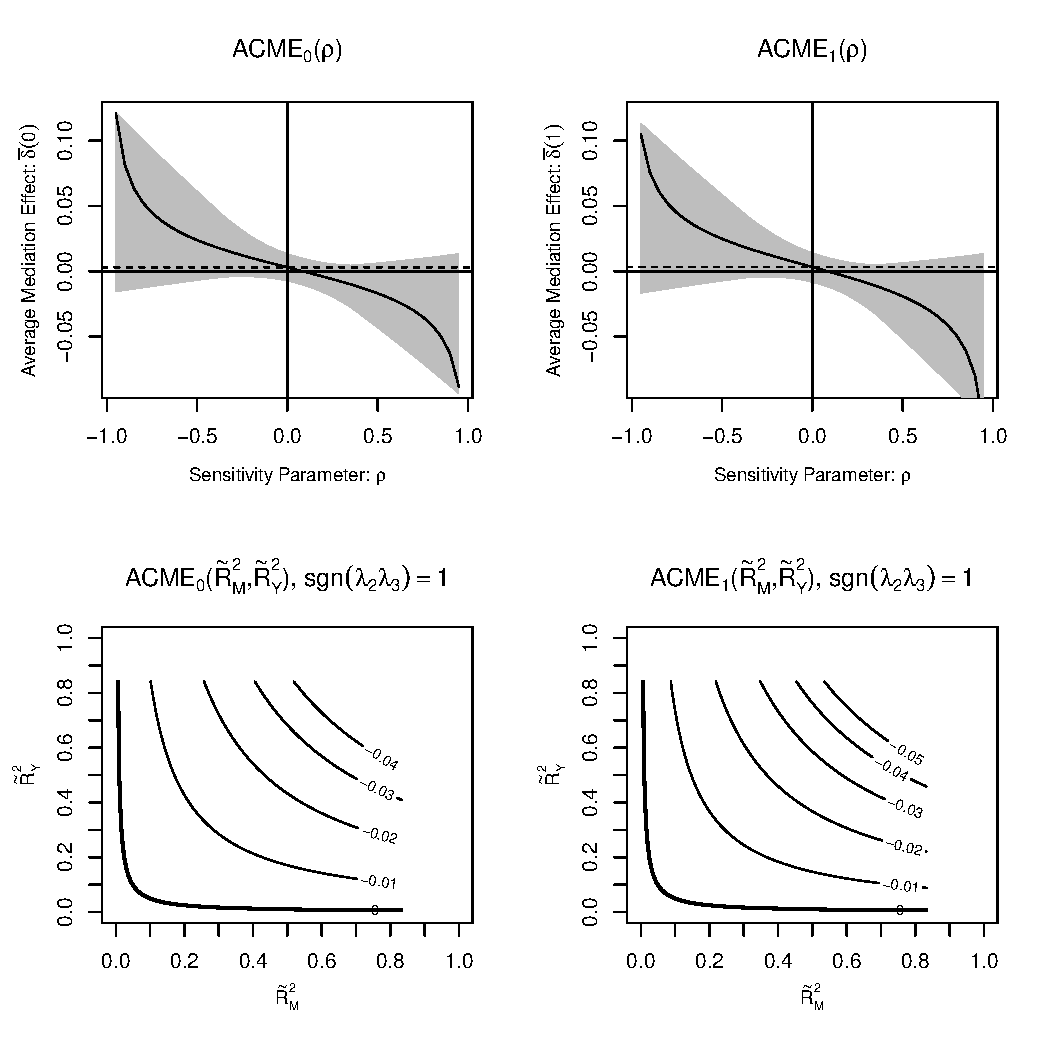
\includegraphics[scale=.8]{Rho-R2-JobsBinOutcome.pdf}
\end{center}
\vspace{-.5in}
\caption{Sensitivity Analysis with Continuous Outcome and Binary Mediator.
  \label{SensBinOut}}
\end{figure}

When the outcome is binary, the proportion of the the total effect due to
mediation can also be calculated as function of the sensitivity parameter $\rho$.
The \texttt{pr.plot} option in the plot command (in conjunction with the
\texttt{sens.par = "rho"} option) allows users to plot a summary
of the sensitivity analysis for the proportion mediated. For example, the
following call would provide a plot of this quantity:
\begin{verbatim}
R> plot(sens.bout, sens.par = "rho", pr.plot = TRUE)
\end{verbatim}


\paragraph{Binary Mediator.}
The final form of sensitivity analysis deals with the case where the
outcome variable is continuous but the mediator is binary.  For the
purpose of illustration, we simply dichotomize the \texttt{job\_seek}
variable to produce a binary measure \texttt{job\_dich}. We fit a
probit model for the mediator and linear regression for the outcome
variable.
\begin{verbatim}
R> model.m <- glm(job_dich ~ treat + depress1 + econ_hard + sex + age 
                + occp + marital + nonwhite + educ + income, 
                data = jobs, family = binomial(link = "probit"))
R> model.y <- lm(depress2 ~ treat + job_dich+ depress1 + econ_hard + sex + age 
                + occp + marital + nonwhite + educ + income, data = jobs)
R> med.bmed <- mediate(model.m, model.y, sims = 1000, treat = "treat",
                       mediator = "job_dich")
R> sens.bmed <- medsens(med.bmed, rho.by = 0.05, sims = 1000)
\end{verbatim}
Again we can pass the output of the \texttt{medsens} function through the \texttt{plot} function,
\begin{verbatim}
R> plot(sens.bmed, sens.par = "rho")
\end{verbatim}
producing Figure \ref{SensBinMed}. The plot is interpreted in the same
way as the above cases. The user also has the option to plot sensitivity results
in terms of the coefficients of determination just as in the case with
continuous outcome and mediator variables.

\begin{figure}[t]
\spacingset{1}
\vspace{-.5in}
\begin{center}
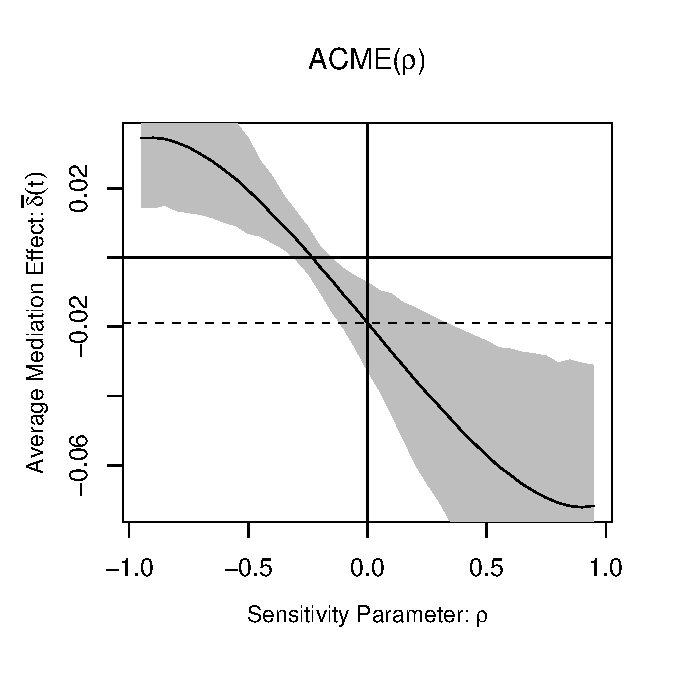
\includegraphics[scale=.8]{BinaryMediator-Sensitivity-Rpaper.pdf}
\end{center}
\vspace{-.5in}
\caption{Sensitivity Analysis with Continuous Outcome and Binary Mediator.
  \label{SensBinMed}}
\end{figure}

When the mediator variable is binary, the plotted values of the mediation effect
and their confidence bands may not be perfectly smooth curves due to simulation errors.
This is especially likely when the number of simulations (\texttt{sims}) is set
to a small value.  In such situations, the user can choose to set the
\texttt{smooth.effect} and \texttt{smooth.ci} options to \texttt{TRUE} in the
\texttt{plot} function so that the corresponding values become smoothed
out via a lowess smoother before being plotted.  Although this option
often makes the produced graph look nicer, the user should be cautious as
the adjustment could affect one's substantive conclusions in a
significant way.  A recommended alternative is to increase the number of
simulations.

\section{Multiple Causal Mediation Analyses via {\tt mediations}}
\label{sec:mediations}
Researchers may face a situation where they want to conduct multiple causal
mediation analyses. For example, the researcher may have run several different
experiments that had different treatment conditions but had the same mediator
and outcome variables. Or, a researcher may measure several different mediating
variables in their experiment and wish to estimate causal mediation effects for
each of these cases. In these situations the researcher would need to write
separate lines of code for the different models. A more efficient way is to
loop over the different combinations of interest.  The {\tt mediations} function
facilitates this process.

The {\tt mediations} function can be used to conduct causal mediation analyses
over the range of treatment, mediator, and outcome combinations that could be
present within a study. For example, if there were two treatment conditions, two
measured mediators, and two outcomes, mediations would run eight causal
mediation analyses. The results can then be analyzed with the {\tt
summary} and {\tt plot} functions. If there is only one
treatment variable, the user needs only a single data set that contains
all mediators and outcomes of interest. If there are multiple treatment
variables, then the researcher must first create separate data frames, each
with all mediator/outcome variables to be considered, and named using a
convention where the name of the data frame object begins with the name of the
treatment variable contained within it.

Use of the {\tt mediations} function is straightforward. First, the user creates
vectors of the treatment, mediator, outcome, and covariates names that are to be used.
The treatment, mediator, and outcome variables are looped over to produce
all possible combinations of mediator and outcome models. The set of covariates
is held constant across the models. The different model combinations are then
entered into the {\tt mediate} function. 

The user can specify several different
options for {\tt mediations}. First, the type of model to be used for the
mediator and outcome equations must be specified. Currently, {\tt mediations} can
handle a variety of different model combinations. Either the mediator or outcome
equation can be modeled with linear regression, probit, ordered probit, and
quantile regression. The {\tt mediations} function also handles the case where tobit is used for
the outcome. Next, the user must also specify the standard features that are necessary for the
{\tt mediate} function, such as the number of simulations ({\tt sims}). In addition, if
quantile regression or tobit regression is used, the user needs to specify 
the appropriate parameters, such as the quantiles to be estimated ({\tt tau.m},
{\tt tau.y}) and cutpoints ({\tt LowerY}, {\tt UpperY}). 
If the user wishes for estimates to include weights
(e.g., survey weights) then the name of the weight variable needs to be passed
via the {\tt weights} argument.

The output of {\tt mediations} contains a collection of {\tt mediate} objects. The naming
system uses the name of the particular outcome variable, mediator, and
treatment, each separated by a dot. For example, if the output of {\tt mediations}
is {\tt output} and the outcome, mediator and treatment variable names
{\tt O}, {\tt M1} or {\tt M2}, and {\tt T}, respectively, 
then {\tt output\$O.M2.T} would be the {\tt mediate} object from using mediator
{\tt M2}.

There are several limitations to the code. First, it works only with a subset of
the model types that will be accommodated if {\tt mediate} is used individually.
Second, one cannot specify separate sets of covariates for different
treatment/mediator/outcome combinations. Users should use {\tt mediate} separately
for individual models if more flexibility is required in their specific
applications. 

While {\tt mediations} is a helpful function, it is also easy to abuse. 
First, researchers must be aware of the assumptions being made at every step of
causal mediation analysis. For example, if there are multiple mediators, a
strong assumption must be made for the estimates to be interpreted as causal
quantities. One such assumption is that the mediators are not causally related. 
Second, care must be taken against the risks of multiple testing when a 
large number of treatment/mediator/outcome combinations are involved.  The
{\tt mediations} function simply runs independent {\tt mediate} processes and
does not use any correction procedures for multiple testing, so the confidence
intervals may be too narrow. We recommend that the use of this function be limited
for exploratory analyses.

An illustration of the {\tt mediations} function can be found in the {\tt Examples}
section of its help document; see {\tt ?mediations} or {\tt example(mediations)}.

\section{Concluding Remarks}

Causal mediation analysis is a key tool for social scientific
research. In this paper, we describe our easy-to-use software for
causal mediation analysis, \bmediation, that implements the new
methods and algorithms introduced by \citet*{imai:keel:yama:10} and
\citet*{imai:keel:ting:10}.  The software provides a flexible, unified
approach to causal mediation analysis in various situations
encountered by applied researchers.  The object-oriented nature of the
\bR\ programming made it possible for us to implement these algorithms
in a fairly general way.  In addition to the estimation of causal
mediation effects, \bmediation\ implements formal sensitivity analyses
so that researchers can assess the robustness of their findings to the
potential violations of the key identifying assumption.  This is an
important contribution for at least two reasons.  First, even in
randomized experiments, causal mediation analysis requires an
additional assumption that is not directly testable from the observed
data.  Thus, researchers must evaluate the consequences of potential
violations of the assumption via sensitivity analysis.  Second, the
accumulation of such sensitivity analyses is essential for
interpreting the relative degree of robustness across different
studies.  Thus, the development of easy-to-use software, such as
\bmediation, facilitates causal mediation analysis in applied social
science research in several critical directions.


\clearpage
\pdfbookmark[1]{References}{References}
\bibliography{my,imai,../../../paper/keele_revised2,../../../paper/TingleyBib}


\end{document}
